\section{Durchführung}
\label{sec:Durchführung}

\begin{figure}
    \centering
    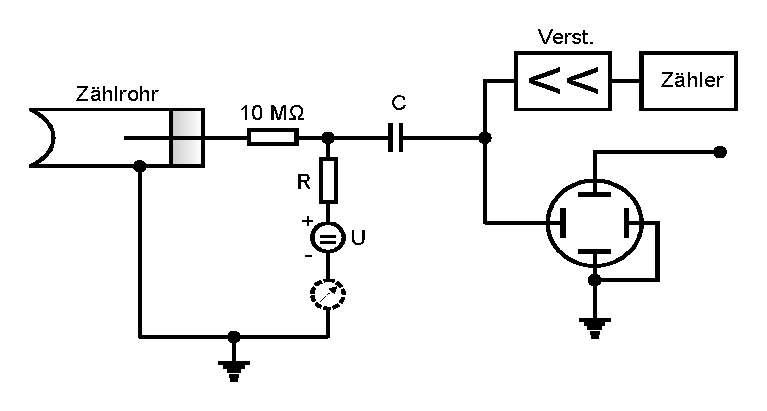
\includegraphics[width=0.5 \linewidth]{pictures/Aufbau2.pdf}
    \caption{Schematischer Aufbau der Messapertur}
    \label{fig:Aufbau2}
\end{figure}

Zunächst wird vom Praktikumsbetreuer die Probe in den Aufbau aus \autoref{fig:Aufbau2} eingesetzt.
Als Probe wird Ti-204 verwendet.
Dann werden alle 120 Sekunden jeweils die Impulse und die Stromstärke abgelesen.
Nach jeden 120 Sekunden wird die Spannung um 10 V erhöht.
Die Messung wird im Bereich 330 V bis 700 V durchgeführt.
700 V ist dabei die obere Grenze, da sonst der Bereich der Dauerentladung erreicht werden würde und so das Zählrohr Schaden nehmen würde.
